\section{Results}

\subsection{Tissue-specific genome-wide gene expression and chromatin accessibility in three tissues}

Gene expression, using RNA-seq, and chromatin accessibility, using ATAC-seq, were measured in lung, liver, and kidney tissues of 47 unique strains in the Collaborative Cross (CC) mouse population. As the function of each tissue is quite distinct, we expected that these data would reflect tissue-specific differences. Principal components analysis (PCA) on each of the gene expression and chromatin accessibility profiles clearly show the clustering of all samples by tissue (\textbf{Figure \ref{fig:pca_plots}}). 

To further validate the quality of these data, we performed pairwise differential expression (DE) and differentially accessible region (DAR) analysis between the three tissues (\textbf{Table \ref{tab:diff_gene}}). We found between 3,564-5,709 DE genes, and 28,048-40,797 DARs across the comparisons. For both expression and chromatin accessibility, liver and kidney tissues were the most similar, and lung and liver were the most distinct, also reflected in the PCA plots. Pathway analyses show between-tissue differences are related mainly to metabolic and immune-related pathways (\textbf{TO DO: Add GSAA tables (FWER < 0.05}) and reflects the distinct demands of each tissue. Energy metabolism pathways were more active in liver and kidney and immune-related pathways were more pronounced in lung. We compared the concordance between DE genes and DARs genome-wide and observed that most DE gene promoters do not show significant differences in chromatin accessibility (\textbf{Figure \ref{fig:diff_concordance}}). In cases where there is significantly variable accessibility in the promoter of a DE gene, though, the vast majority agree in direction (i.e. higher expression and greater accessibility). Together, these results support the high quality of the gene expression and chromatin accessibility data.

\begin{figure*}[h]
\renewcommand{\familydefault}{\sfdefault}\normalfont
\centering
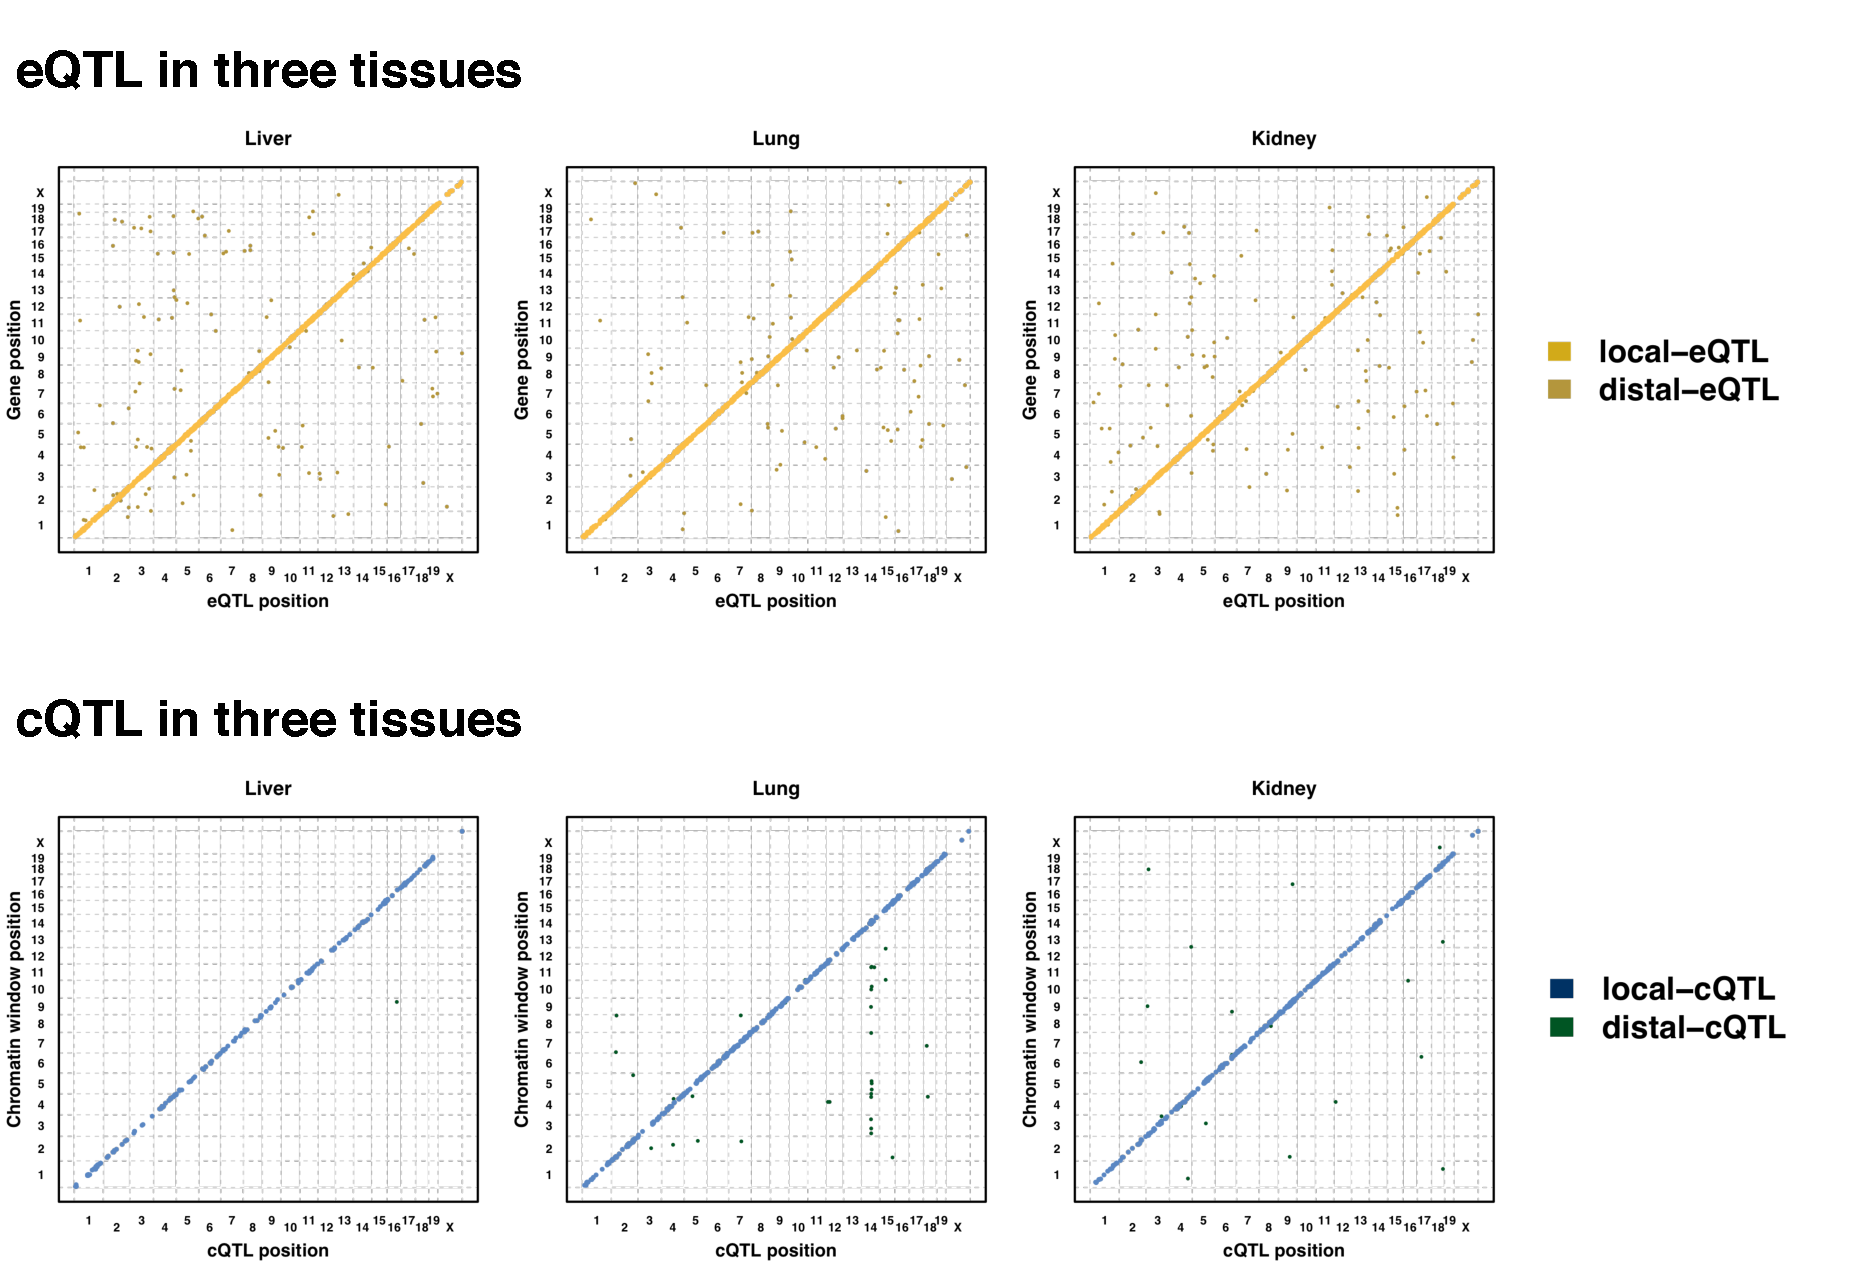
\includegraphics[width=\textwidth, trim={0in 0in 0in 0in}, clip]{figs/qtl_map_main.pdf}
\caption{\textbf{Detected QTL are largely local for both gene expression and chromatin accessibility.} Detected QTL from Method 1 (multi-stage FDR) and Method 3 (genome-wide and chromosome-wide) are included, excluding intra-chromosomal distal-QTL detected through Method 2. The y-axis represents the genomic position of the gene or chromatin site, and the x-axis represents the genomic position of the QTL. Local-QTL appear as dots along the diagonal, and distal-QTL off of it.
\label{fig:grid_plot}}
\end{figure*}

\subsection{Tissue-specific expression QTL}

To evaluate the impact of genetic variation on gene expression, three approaches to detect eQTL were used (\textbf{Table \ref{tab:qtl_procedures}}), summarized here and described more completely in \textbf{Appendix B}. Method 1 was the most stringent and involved a multi-stage conditional regression procedure paired with an FDR control that allowed for the detection of potentially multiple eQTL per gene and requiring significance at a genome-wide level. Method 2 required FDR-controlled significance at the less stringent chromosome-wide level and only used results from the first stage of the multi-stage analysis, which we refer to as a single-step analysis. Method 3 was also a single-step analysis and employed an even more lenient significance criteria based on the genome-wide and chromosome-wide adjusted FWER p-value. We classified local-eQTL as being within 10 Mb of the transcription start site (TSS) of the gene, and distal-eQTL as being greater than 10 Mb from the TSS on the same chromosome (intra-chromosomal) or on a different chromosome (inter-chromosomal). For Method 2, only local-eQTL and intra-chromosomal distal-eQTL were detected due to our use of chromosome-wide significance criteria. For Method 3, the least stringent method, we only detected local-eQTL.

After filtering lowly expressed genes, a total of 8401, 11357, and 10092 genes were considered for liver, lung, and kidney tissues, respectively. Positions of local-eQTL detected for each tissue using any of the three methods (Method 1, genome-wide q-value < 0.1; Method 2, chromosome-wide q-value < 0.1; Method 3, genome-wide and chromosome-wide FWER p-value < 0.05)  are shown in \textbf{Figure \ref{fig:grid_plot} [top]} (light colored dots), as well as summarized in \textbf{Table \ref{tab:eqtl_mapping}}. We also identified eQTL with Method 1 using a more relaxed significance threshold (q-value < 0.2; \textbf{Table \ref{tab:eqtl_mapping_lenient}}). Increasing the FDR threshold from 0.1 to 0.2 increases the number of distal-eQTL detected to a greater extent than local-eQTL. Using Method 3 and requiring genome-wide significance, the percentage of tested genes with local-eQTL are 6.3\%, 8.4\%, and 9.5\% for lung, liver, and kidney, respectively (\textbf{Table \ref{tab:eqtl_mapping}}). These percentages increase to 16.6\%, 19.8\%, and 20.8\% when criteria were less stringent with only chromosome-wide significance. 

For each eQTL detected by any of our methods, we estimated the effect size of the eQTL by two methods (see \textbf{Tables XX}), either the coefficient of determination ($R^{2}$) for the fixed effect fitting of the QTL term (\textbf{Methods}; Eq \ref{eq:effect_size}) or as the proportion of variance explained based on the variance component estimate from a random effect fitting of the QTL term (\textbf{Methods}; Eq \ref{eq:effect_size_ranef}). We primarily report results from the fixed effect approach because the estimates were largely consistent with plausible QTL effect sizes given the size of the study, outlined in \cite{KeeleSPARCC}, namely we were not well-powered to detect QTL with effect sizes < 50\% at genome-wide significance. As expected, Method 1 detects eQTL with large effects (\textbf{Figure \ref{fig:qtl_effect_sizes_by_method}}, red dots). The less stringent Methods 2 and 3 result in greater power to detect local-eQTL with reduced effects (\textbf{Figure \ref{fig:qtl_effect_sizes_by_method}}, gray and blue dots). Distal-eQTL discovered with the multi-stage mapping procedure (Method 1; q-value < 0.1) were detected for $\leq$ 1.6\% of tested genes (\textbf{Table \ref{tab:eqtl_mapping}}; \textbf{Figure \ref{fig:grid_plot} [top]}, dark colored dots), and, consistent with previous studies (\textit{eg} \citealt{Chick2016}), have weaker effects than local-eQTL (\textbf{Figure \ref{fig:qtl_effect_sizes_strict} [top]}). For both Methods 1 and 2, almost three times as many local-eQTL are detected compared to distal-eQTL, likely reflecting these stronger effects. For some distal-eQTL, the effect sizes estimated through random effects models approach zero, potentially resulting from highly influential data points in the fixed effect regression procedure and are thus likely to be false positives (\textbf{Figure \ref{fig:qtl_effect_size_fixefvsranef}}). 

To assess whether distance measures to classify intra-chromosomal local- vs distal-eQTL were reasonable, we plotted the statistical association for all intra-chromosomal eQTL from Method 1 (\textbf{Figure \ref{fig:genomewide_dist} [top]}) and the less stringent Method 2 (\textbf{Figure \ref{fig:chrwide_dist} [top]}). In addition to finding that the majority are local-eQTL, we see a drastic reduction in the strength of the statistical association outside of the defined local region. This suggests that intra-chromosomal distal-eQTL are more similar to inter-chromosomal distal-eQTL than local-eQTL, and that our 10Mb boundaries are appropriate. 

Founder allele effects were estimated for all eQTL, using a random effects model to constrain unstable estimates. Consistent with previous studies (\eg \citealt{Aylor2011}), the CAST and PWK alleles tended to have more extreme effects than the classical inbred strains. This pattern was observed for both local and distal eQTL (\textbf{Figure \ref{fig:eqtl_effects_abs}}).

\subsection{Tissue-specific chromatin QTL}

To determine genetic effects on chromatin structure, genomic regions were divided into $\sim$300 base pair windows, and used in chromatin accessibility QTL (cQTL) analysis with the same methods used for eQTL. We tested 11448, 24426, and 17918 chromatin regions in liver, lung, and kidney, respectively. Overall, there were substantially fewer cQTL detected compared to eQTL for all tissues (\textbf{Figure \ref{fig:grid_plot} [bottom]};\textbf{Table \ref{tab:cqtl_mapping}}). As with eQTL, cQTL are more likely to be local (66\%-94.1\% for Method 1; 75\%-90\% for Method 2).
Consistent with eQTL, the effect sizes of local-cQTL are on average higher than distal-cQTL (\textbf{Figure \ref{fig:qtl_effect_sizes_strict} [bottom]}), likely contributing to the to the small number of detected distal-cQTL. cQTL with low effect size are primarily distal-cQTL and may represent false positives. Likewise, most intra-chromosomal cQTL detected using Method 1 or 2 are local-cQTL, and the significance of association is much greater for the local-cQTL  (\textbf{Figure \ref{fig:genomewide_dist} [bottom]} and \textbf{Figure \ref{fig:chrwide_dist} [bottom]}).
Again we found that the CAST and PWK founder alleles have more extreme effects than the other strains for local-cQTL, though the pattern is less pronounced than with local-eQTL, likely due to the reduced number of cQTL (\textbf{Figure \ref{fig:cqtl_effects_abs}}). The numbers of detected distal-cQTL are low, and no clear trends are obvious.

\section{Paired QTL detected in multiple tissues}

For a given trait, QTL from different tissues were paired based on co-localizing to approximately the same genomic region. For local-QTL, both had to be within the local window, defined at 10 Mb around the gene TSS, resulting in a maximum distance of 20 Mb between QTL. For distal-eQTL, both had to be within 10 Mb of each other. 
For local-eQTL, 761 (liver/lung), 1206 (liver/kidney), and 1025 (lung/kidney) pairs were detected. With distal-eQTL, 61 (liver/lung), 120 (liver/kidney), and 59 (lung/kidney) were identified. For cQTL, the vast majority of pairs were local, with 55 (liver/lung), 56 (liver/kidney), and 142 (lung/kidney). Only 4 distal-cQTL pairs were observed, all between lung and kidney. The effect sizes of paired QTL vary across tissues, though they were significantly correlated (\textbf{Figure \ref{fig:qtl_effect_size_comparison}}).

Correlations between the founder allele effects for pairs of QTL were calculated (FDR $\le 0.1$; \textbf{Figures \ref{fig:qtl_pair_histograms}}), with 345 (liver/lung), 623 (liver/kidney), and 498 (lung/kidney) local-eQTL pairs and 21 (liver/lung), 34 (liver/kidney), and 16 (lung/kidney) distal-eQTL pairs positively correlated. Highly correlated QTL pairs were highly proximal to each other (\textbf{Figure \ref{fig:qtl_cor_by_distance_comparison}}), suggesting that the underlying causal variants are the same or linked. 47 (liver/lung), 48 (liver/kidney), and 118 (lung/kidney) positively correlated local-cQTL pairs. The correlations between distal-cQTLs were not formally tested because there were only four pairs; however, three of the four pairs had correlations greater than 0.5. No negatively correlated QTL pairs were detected, after accounting for multiple testing.

\begin{figure*}[h!]
\renewcommand{\familydefault}{\sfdefault}\normalfont
\centering
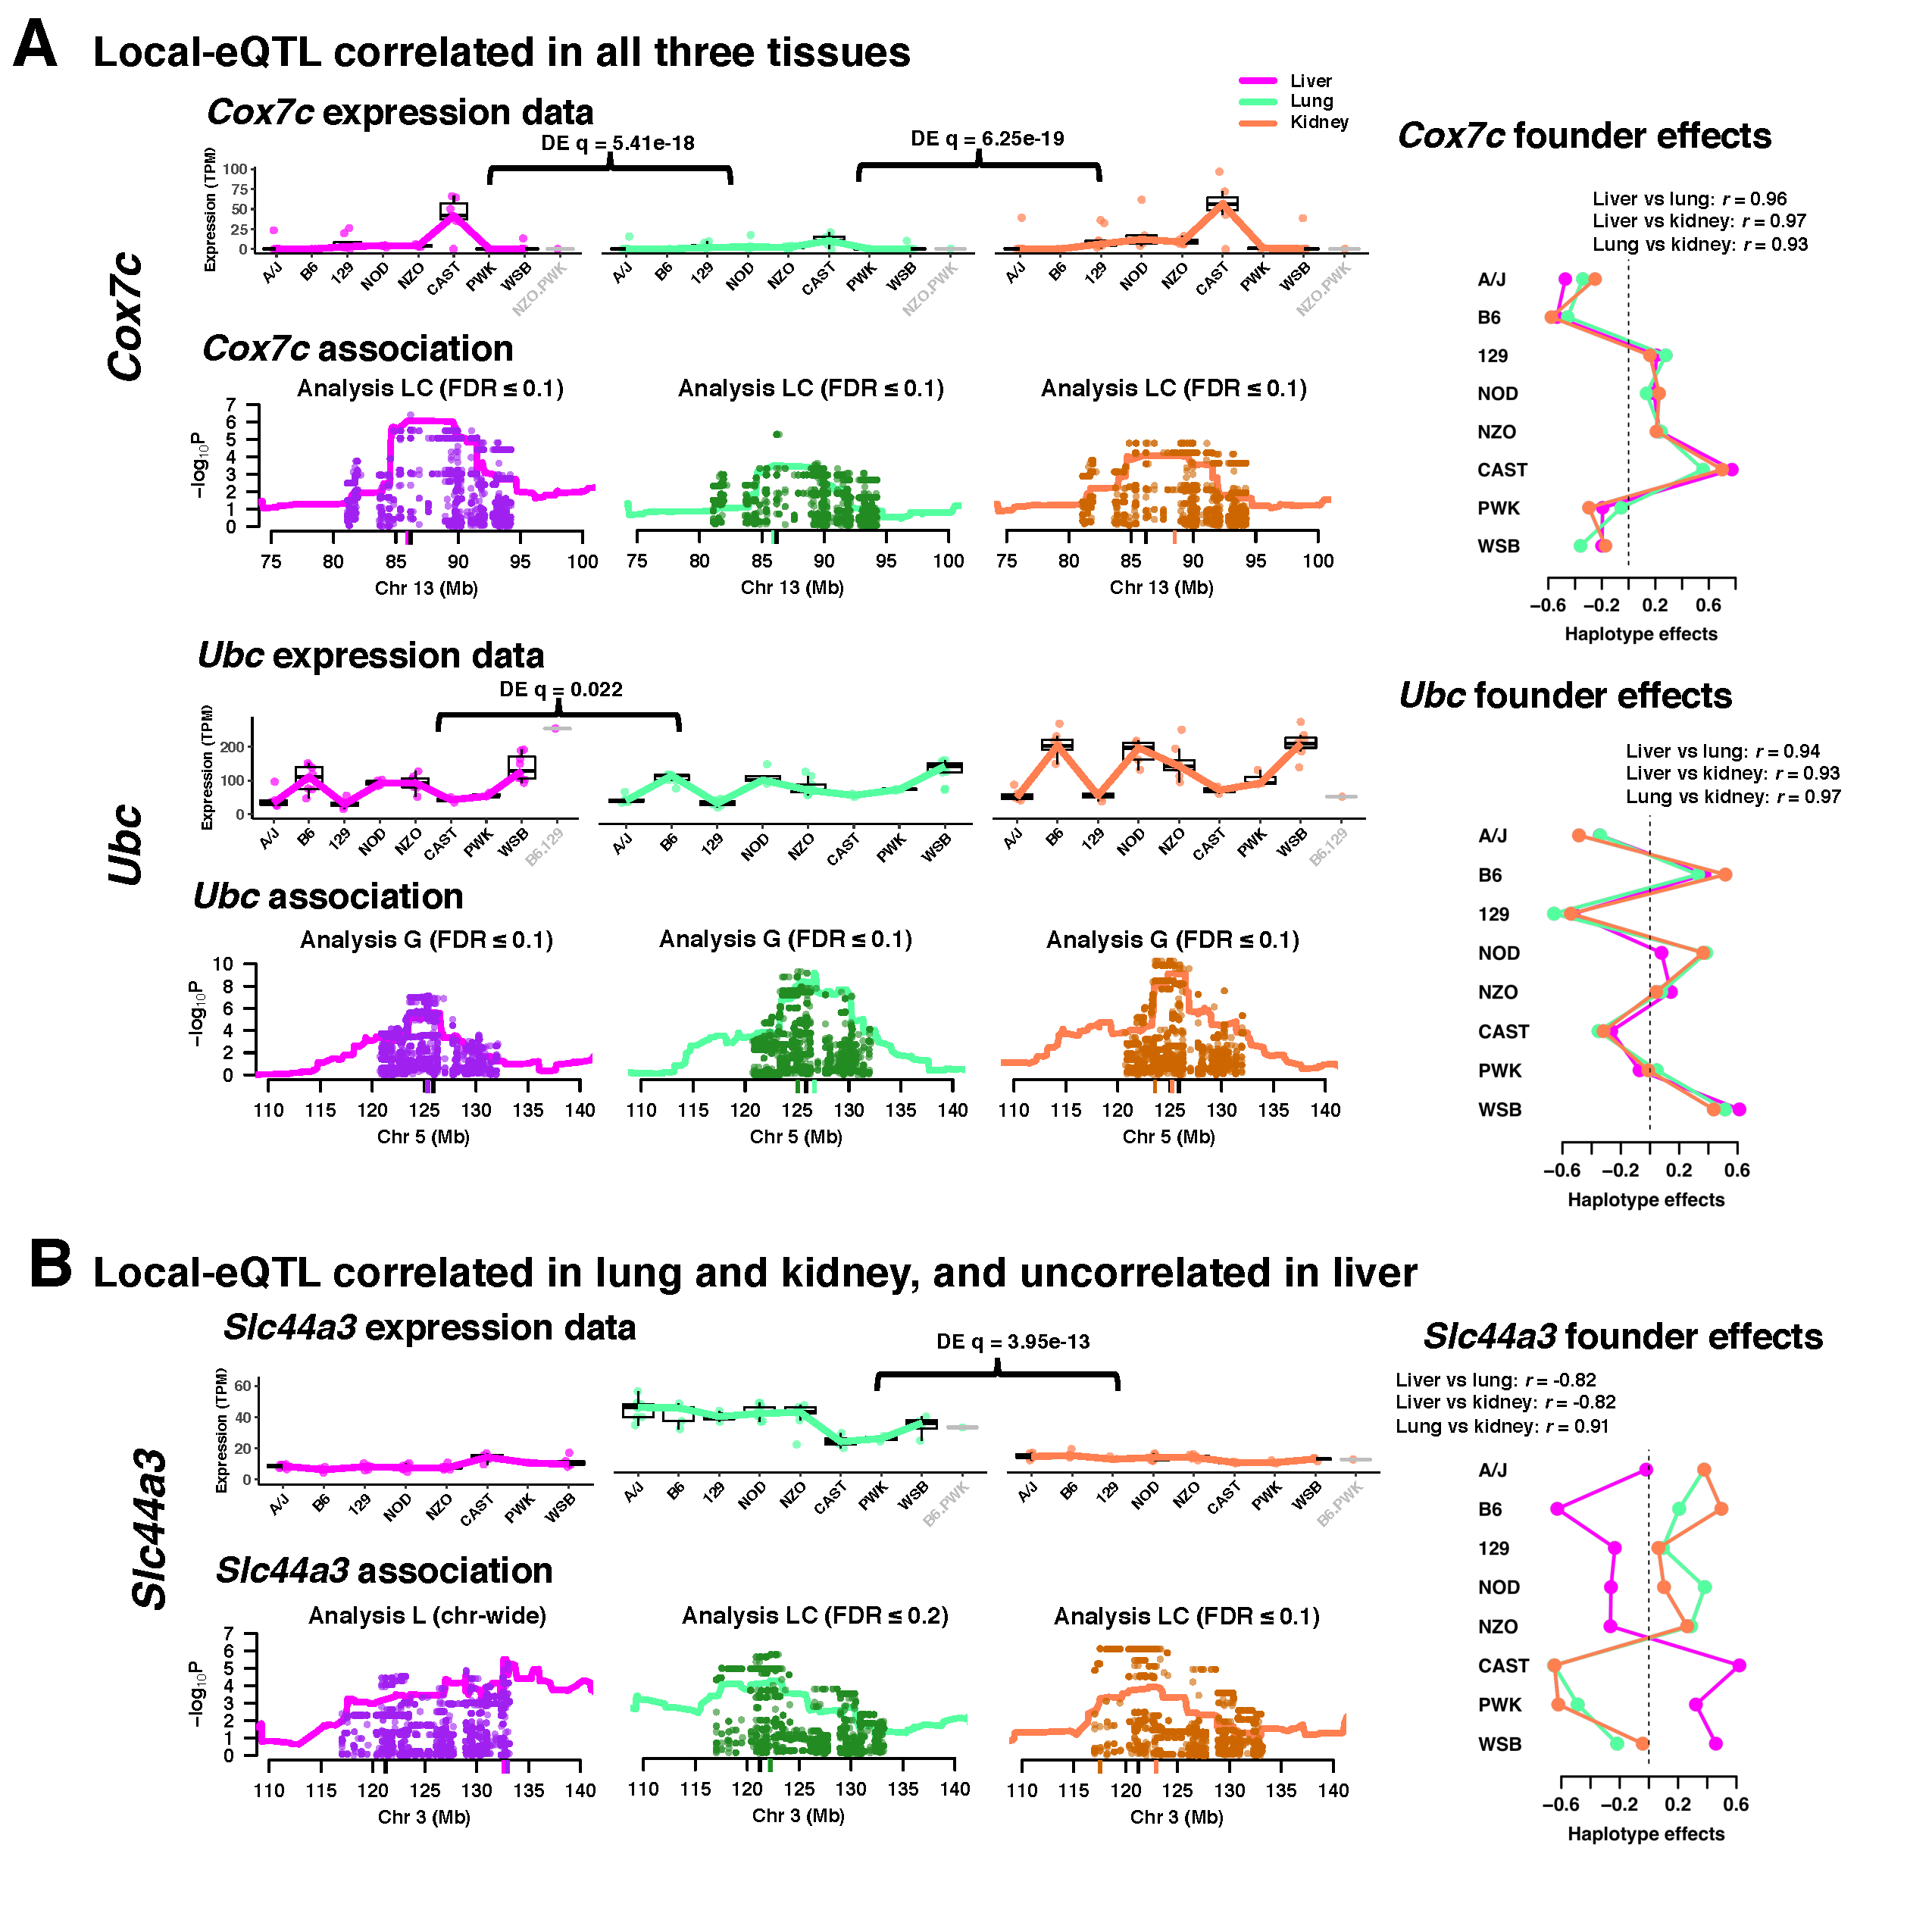
\includegraphics[width=0.9\textwidth, trim={0in 0.5in 0in 0in}, clip]{figs/correlated_local_eqtl.pdf}
\caption{\textbf{Examples of genes with local-eQTL observed in all three tissues.} \textit{Cox7c} and \textit{Ubc} possess local-eQTL with highly correlated founder alllele effects across all three tissues, supportive of shared causal origin (A). \textit{Slc44a3} has a more complicated pattern of local-eQTL founder effects across the tissues, with correlated effects shared between lung and kidney, and transgressive effects in the liver eQTL by comparison, consistent with distinct casual variants comparing liver to lung and kidney. (B). For each gene, the expression data is plotted with boxplots based on most likely founder haplotype pair (diplotype), and differential expression between tissues is highlighted. The haplotype association for each tissue is also included near the gene TSS with variant association overlaid. The most statistically rigorous method to detect the QTL is also included. The black tick represents the gene TSS and the colored ticks represent haplotype and variant peaks. Founder effects estimated as constrained BLUPs are also included with their pairwise correlations. Estimated effects were generally consistent with the expression data.\label{fig:correlated_local_eqtl}}
\end{figure*}

%\subsection{Genes with correlated local-eQTL: \textit{Cox7c} and \textit{Ubc}}

Cytochrome c oxidase subunit 7C (\textit{Cox7c}) and ubiquitin C (\textit{Ubc}) are examples of genes that possess local-eQTL with highly correlated effects in all three tissues (\textbf{Figure \ref{fig:correlated_local_eqtl}A}).
For \textit{Cox7c} local-eQTL were driven by high expression when the CAST allele was present, intermediate expression with 129, NOD, and NZO alleles, and low expression with A/J, B6, PWK, and WSB alleles. The \textit{Ubc} local-eQTL were driven by high expression with the B6, NOD, NZO, and WSB alleles. Though the founder effects are consistent across tissues for both genes, we note that expression of \textit{Cox7c} was significantly higher in liver compared to both lung ($q = \num{5.41e-18}$) and kidney ($q = \num{6.25e-19}$), and for \textit{Ubc}, expression in liver and lung were considered significantly differential ($q = 0.022$). 

%The haplotype and variant associations in the local region match closely for all tissues for both \textit{Cox7c} and \textit{Ubc}. Though all the \textit{Ubc} local-eQTL were detected with the most stringent Method 1, the \textit{Cox7c} local-eQTL were detected with the more lenient Method 2.

%\subsection{Genes with uncorrelated local-eQTL: \textit{Slc44a3} and \textit{Pik3c2g}}

\begin{figure*}[h]
\renewcommand{\familydefault}{\sfdefault}\normalfont
\centering
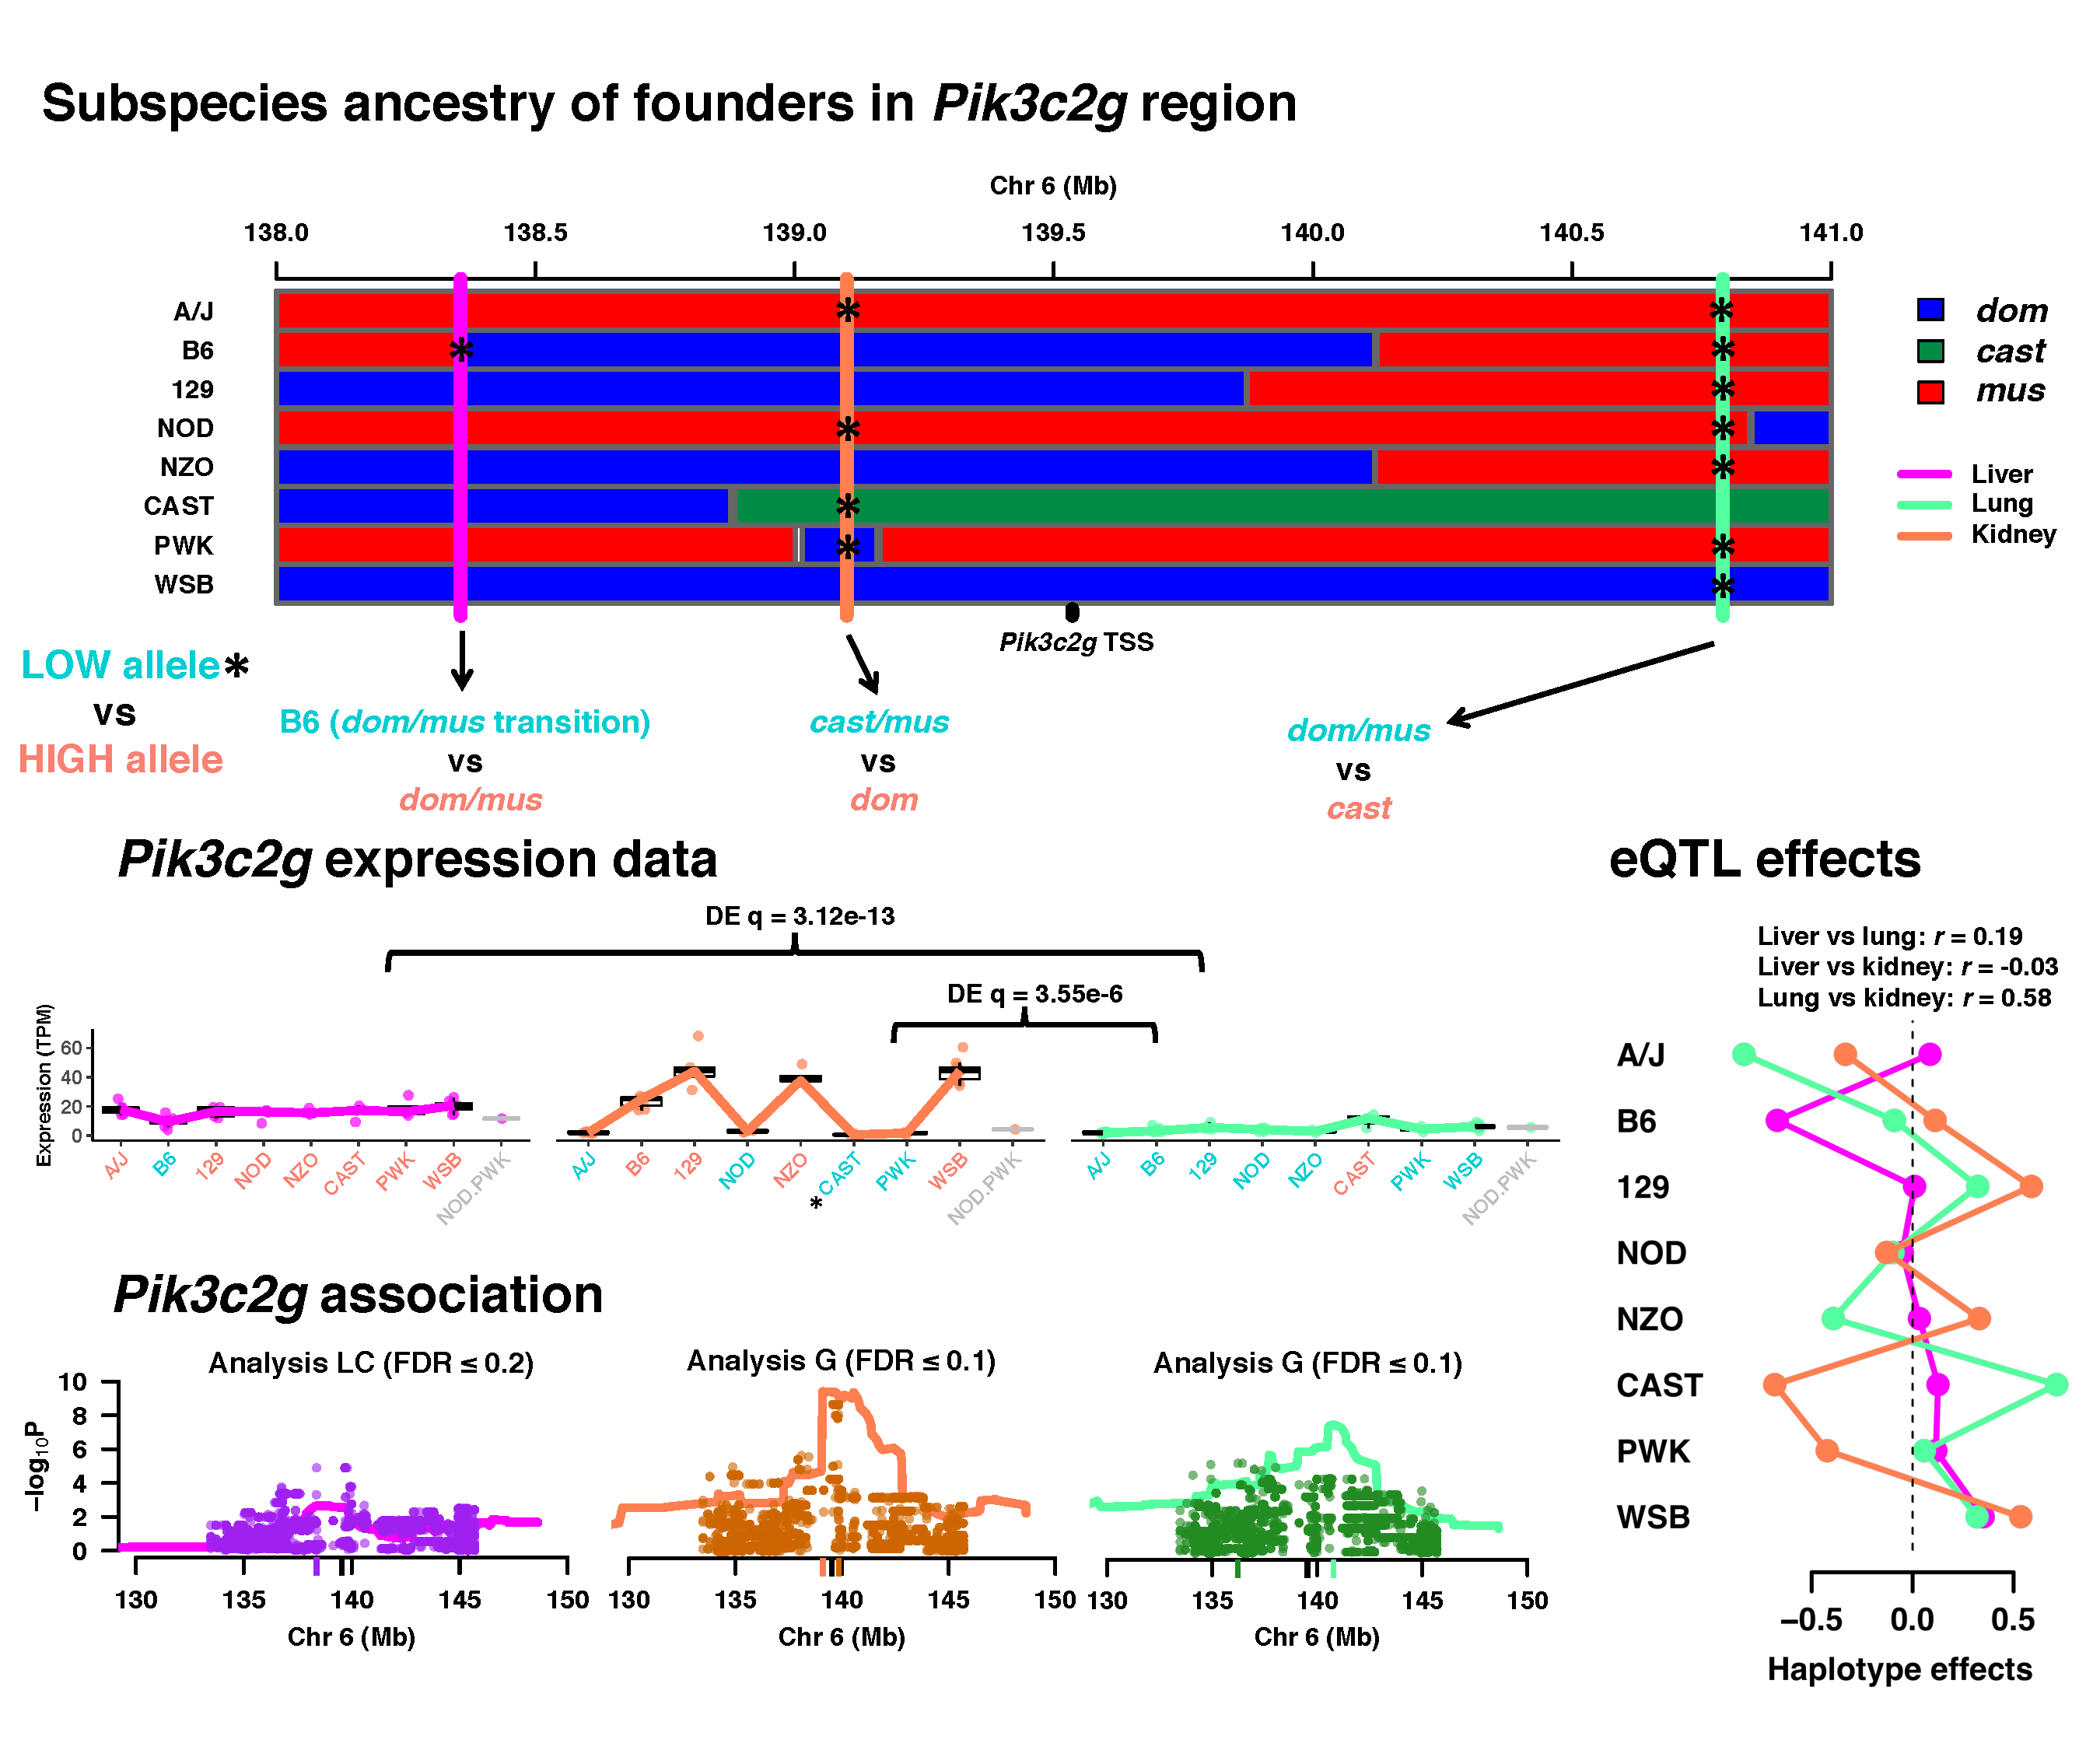
\includegraphics[width=0.9\textwidth, trim={0in 0.5in 0in 0in}, clip]{figs/pik3c2g_example.pdf}
\caption{\textbf{\textit{Pik3c2g} possesses tissue-specific local-eQTL.} Local-eQTL for \textit{Pik3c2g} are detected in all three tissues in the 3Mb region surrounding its TSS. The genomes of the CC founders can be simplified in terms of contributions from three subspecies lineages of \textit{M. musculus}: \textit{dom} (blue), \textit{cast} (green), and \textit{mus} (red). The effects of each local-eQTL matched the subspecies contributions near the eQTL coordinates, with low subspecies alleles colored teal and high alleles colored salmon, consistent with local-eQTL for \textit{Pik3c2g} being distinct and tissue-specific. The gene expression data is represented as boxplots, categorized based on most likely diplotype at the eQTL for each CC strain. Haplotype and variants associations are included for each tissue, with the black tick representing the \textit{Pik3c2g} TSS and colored ticks representing haplotype and variant peaks. The most rigorous procedure to detect each QTL is reported. Founder effects, estimated as constrained BLUPs, were consistent with the expression data, and uncorrelated across the tissues.\label{fig:pik3c2g}}
\end{figure*}

QTL pairs that are uncorrelated potentially represent distinct tissue-specific QTL where genetic variants influence gene expression or chromatin accessibility in a tissue-specific pattern. For example, the solute carrier family 44, member 3 (\textit{Slc44a3}) gene has correlated local-eQTL effects in lung and kidney, but unique effects in liver (\textbf{Figure \ref{fig:correlated_local_eqtl}B}). Notably, the effects in liver are anti-correlated with the effects in lung and kidney, suggesting the liver eQTL could be transgressive \citep{Rieseberg1999} to the eQTL in lung and kidney, whereby the effects of the founder alleles are reversed. For \textit{Slc44a3}, CAST, PWK, and WSB alleles result in higher expression in liver, but lower expression in lung and kidney. 
The local-eQTL for \textit{Slc44a3} were more similar in location in lung and kidney, whereas the liver eQTL was more distal to the gene TSS. Overall, the expression data, estimated effects, and patterns of association are consistent with lung and kidney sharing a causal local-eQTL, and liver possessing a unique one. 
%The lung eQTL was detected with the highly lenient Method 2 (FDR $\leq$ 0.2) and the kidney eQTL with the less lenient Method 2 (FDR $\leq$ 0.1). The liver eQTL was detected with the lenient Method 3 (chromosome-wide). 

Another example is phosphatidylinositol-4-phosphate 3-kinase catalytic subunit type 2 gamma (\textit{Pik3c2g}), a gene of interest for diabetes-related traits \citep{Braccini2015}. \textit{Pik3c2g} has local-eQTL in all three tissues but that are all uncorrelated (\textbf{Figure \ref{fig:pik3c2g}}). Expression of \textit{Pik3c2g} varies at statistically significant levels for liver versus lung ($q = \num{3.12e-13}$) and lung versus kidney ($q = \num{3.55e-6}$). The presence of tissue-specific local-eQTL is further supported by the \textit{Mus musculus} lineages in the genomic region local to \textit{Pik3c2g}. The CC founder strains all possess contributions from three subspecies of \textit{M. musculus}: \textit{domesticus} (\textit{dom}), \textit{castaneus}, (\textit{cast}), and \textit{musculus} (\textit{mus}) \citep{Yang2011}. \cite{Crowley2015} found that allele-specific gene expression in mice descended from the CC founders often followed patterns that matched the subspecies inheritance at the gene regions.
In lung, the CAST allele, which represents the \textit{cast} subspecies lineage at the locus, results in higher expression, consistent with a \textit{cast} versus \textit{dom}/\textit{mus} allelic series. In kidney, the B6, 129, NZO, and WSB alleles result in higher expression, whereas A/J, NOD, CAST, and PWK alleles show almost no expression, mostly consistent with a \textit{dom} versus \textit{cast}/\textit{mus} allelic series. The PWK founder has a small \textit{dom} haplotype block at the QTL peak in a broader region that is largely \textit{mus}. The expression data are highly consistent with PWK having the \textit{mus} allele, suggesting that the causal variant is located in a nearby region, supported by the variant association. Notably, the B6 allele expression appears intermediate to the other founders that possess \textit{dom} inheritance, representing a potentially multi-allelic QTL that haplotype association can better identify in comparison to bi-allelic variant association. In liver, the B6 allele resulted in lower expression. The B6 founder does not have a unique subspecies lineage at the locus, but instead possesses a recombination event between \textit{dom} and \textit{mus}, potentially disrupting the local regulation specific to each subspecies lineage and explaining the reduced expression.

%\subsection{Genes with distal-QTL observed across tissues: \textit{Akr1e1}, \textit{Per2}, and \textit{Rnf13}}

\begin{figure*}[h!]
\renewcommand{\familydefault}{\sfdefault}\normalfont
\centering
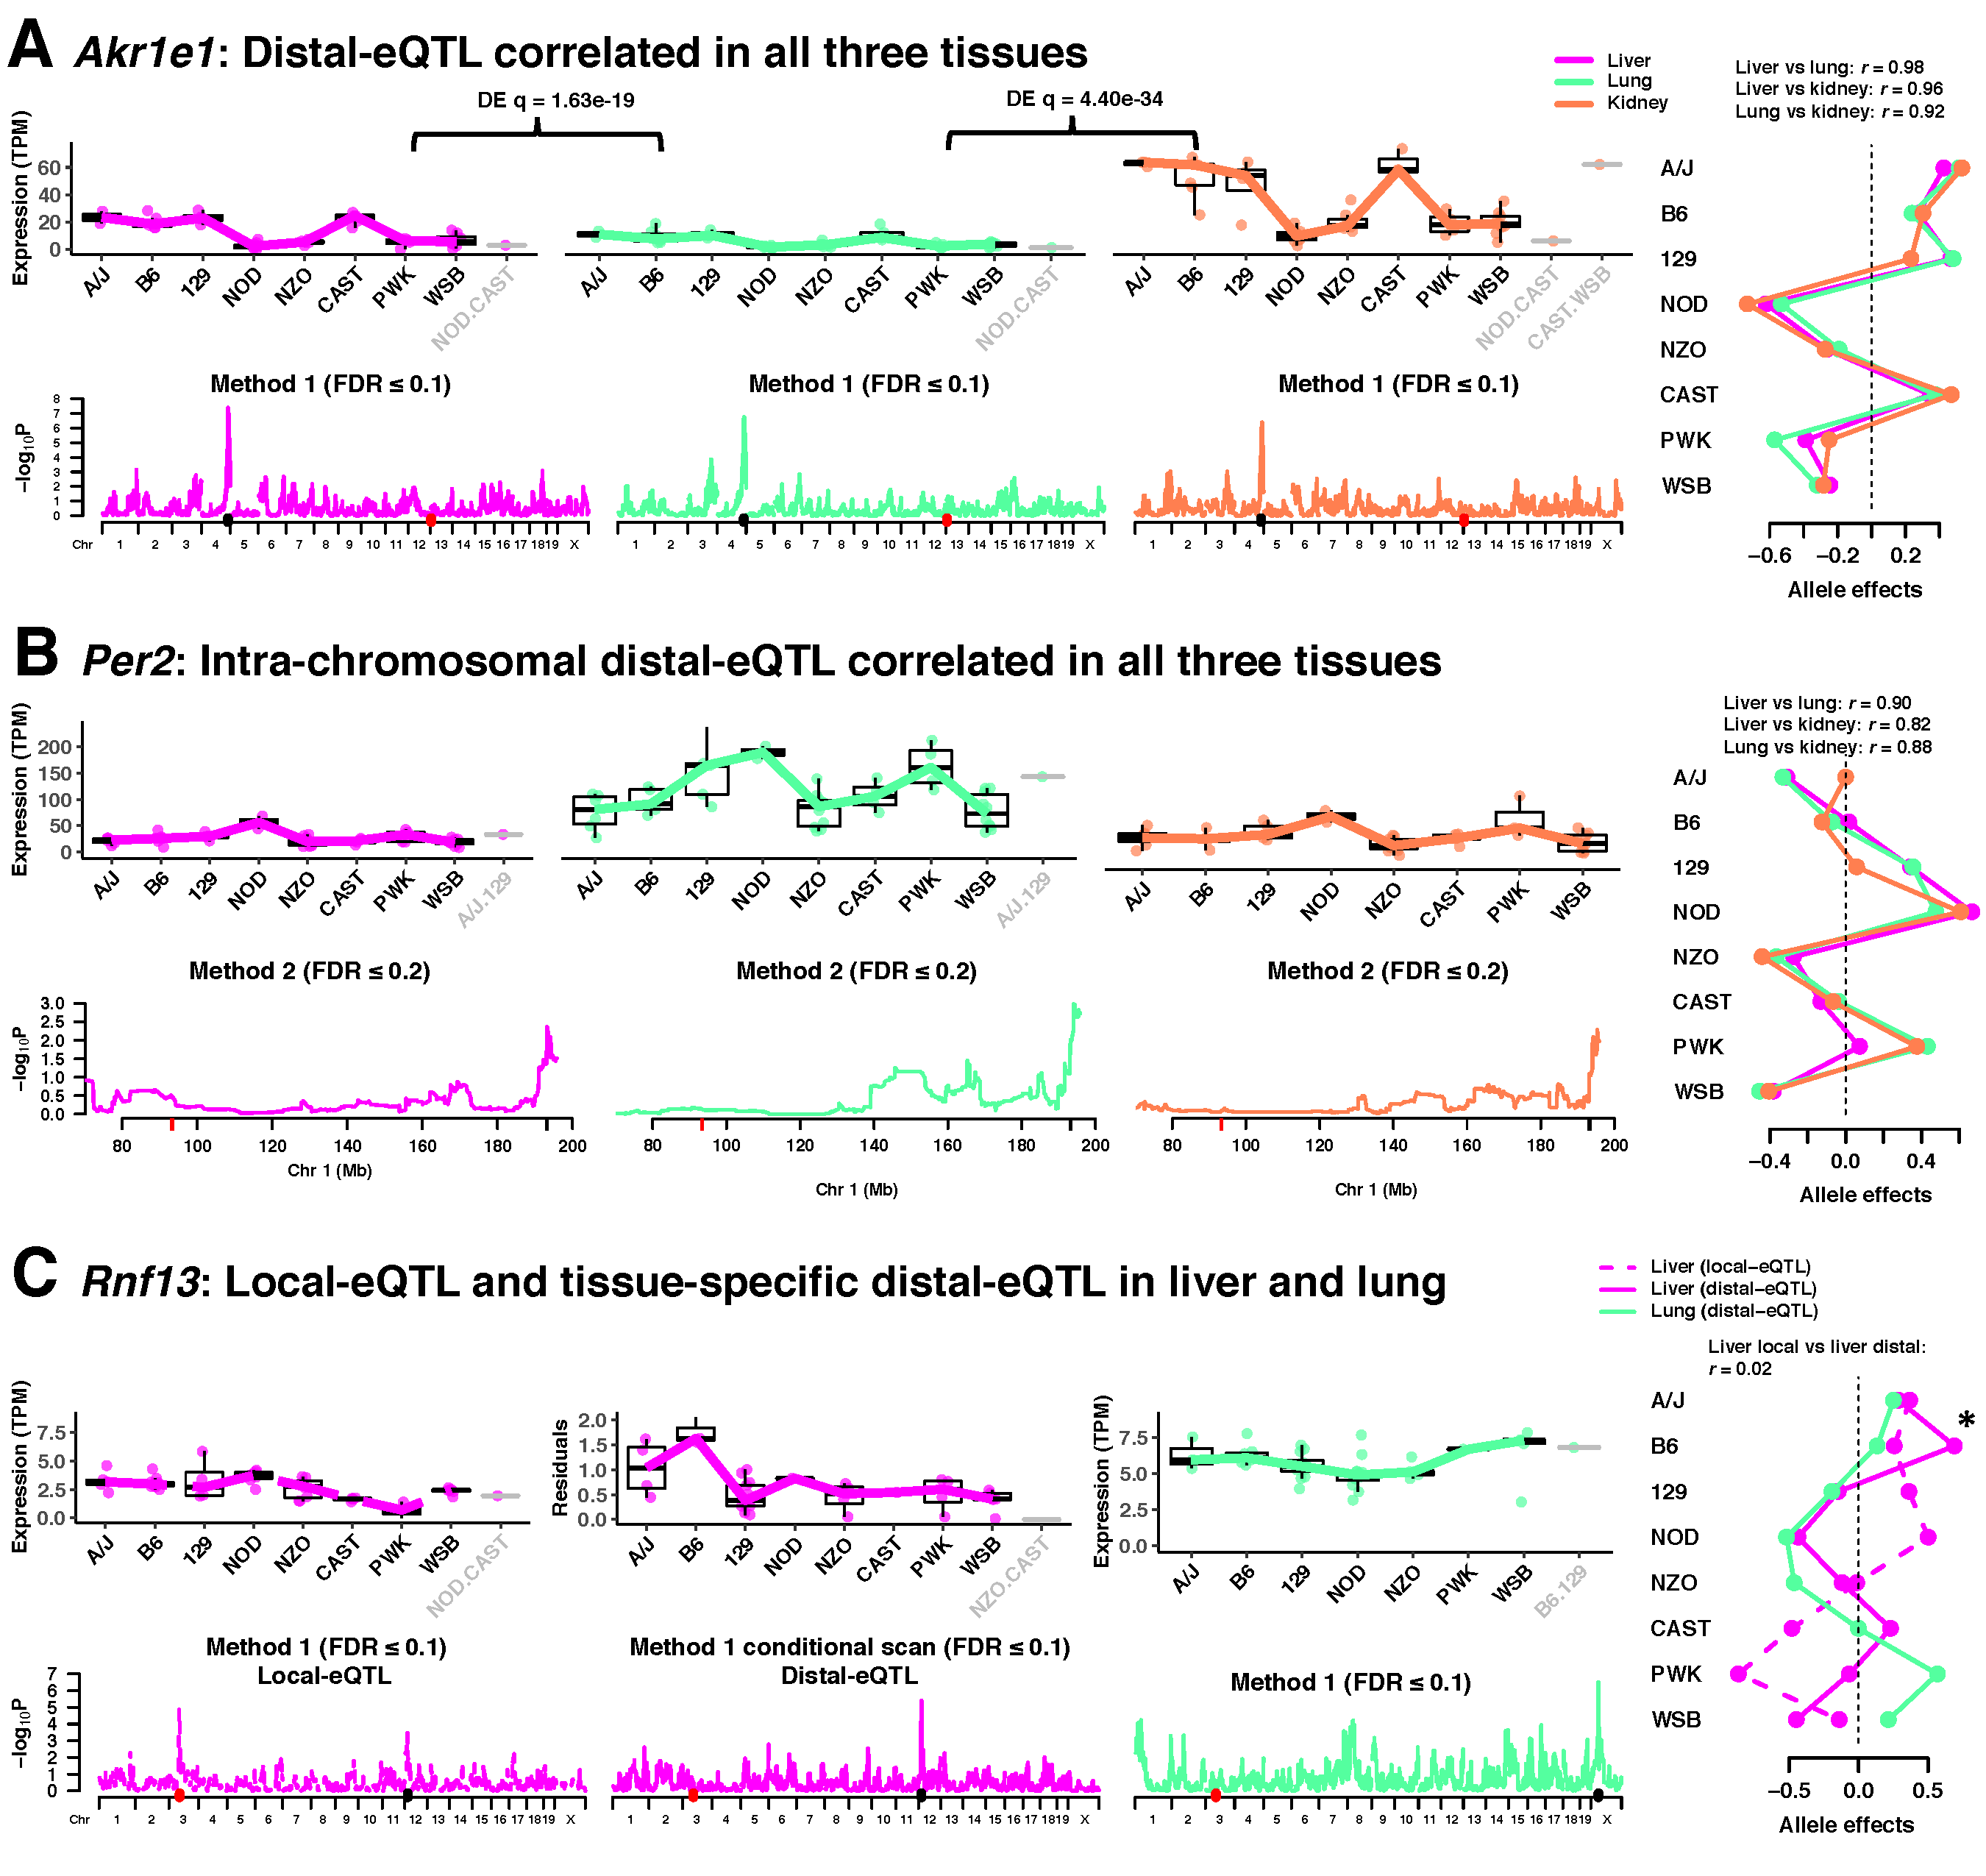
\includegraphics[width=0.9\textwidth, trim={0in 0in 0in 0in}, clip]{figs/correlated_distal_eqtl.pdf}
\caption{\textbf{Examples of genes with distal-eQTL effect patterns across tissues.} \textit{Akr1e1} has highly significant distal-eQTL detected on chromosome 4 in all three tissues with correlated founder effects (A). \textit{Per2} has intra-chromosomal distal-eQTL leniently detected 100Mb away from the TSS, also with highly correlated founder effects across the tissue, providing further support that the distal-eQTL are real (B). \textit{Rnf13} has a liver-specific distal-eQTL on chromosome 12 detected after conditioning on its local-eQTL on chromosome 2, and a lung-specific distal-eQTL on chromosome X, each with distinct founder effect patterns (C). Expression data are represented as boxplots for most likely diplotype, with differential expression noted when significant. Haplotype associations for each tissue distal-eQTL combination are shown, with the most rigorous statistical procedure for detection reported. Red ticks signify the gene TSS and black ticks represent that eQTL peak. Fit founder effects, estimated as BLUPs, are included, along with the pairwise correlations of the eQTL. The black asterisk marks the high B6 effect that drives the distal-eQTL in liver after conditioning on the local-eQTL for \textit{Rnf13}.
\label{fig:correlated_distal_eqtl}}
\end{figure*}

\begin{figure*}[h]
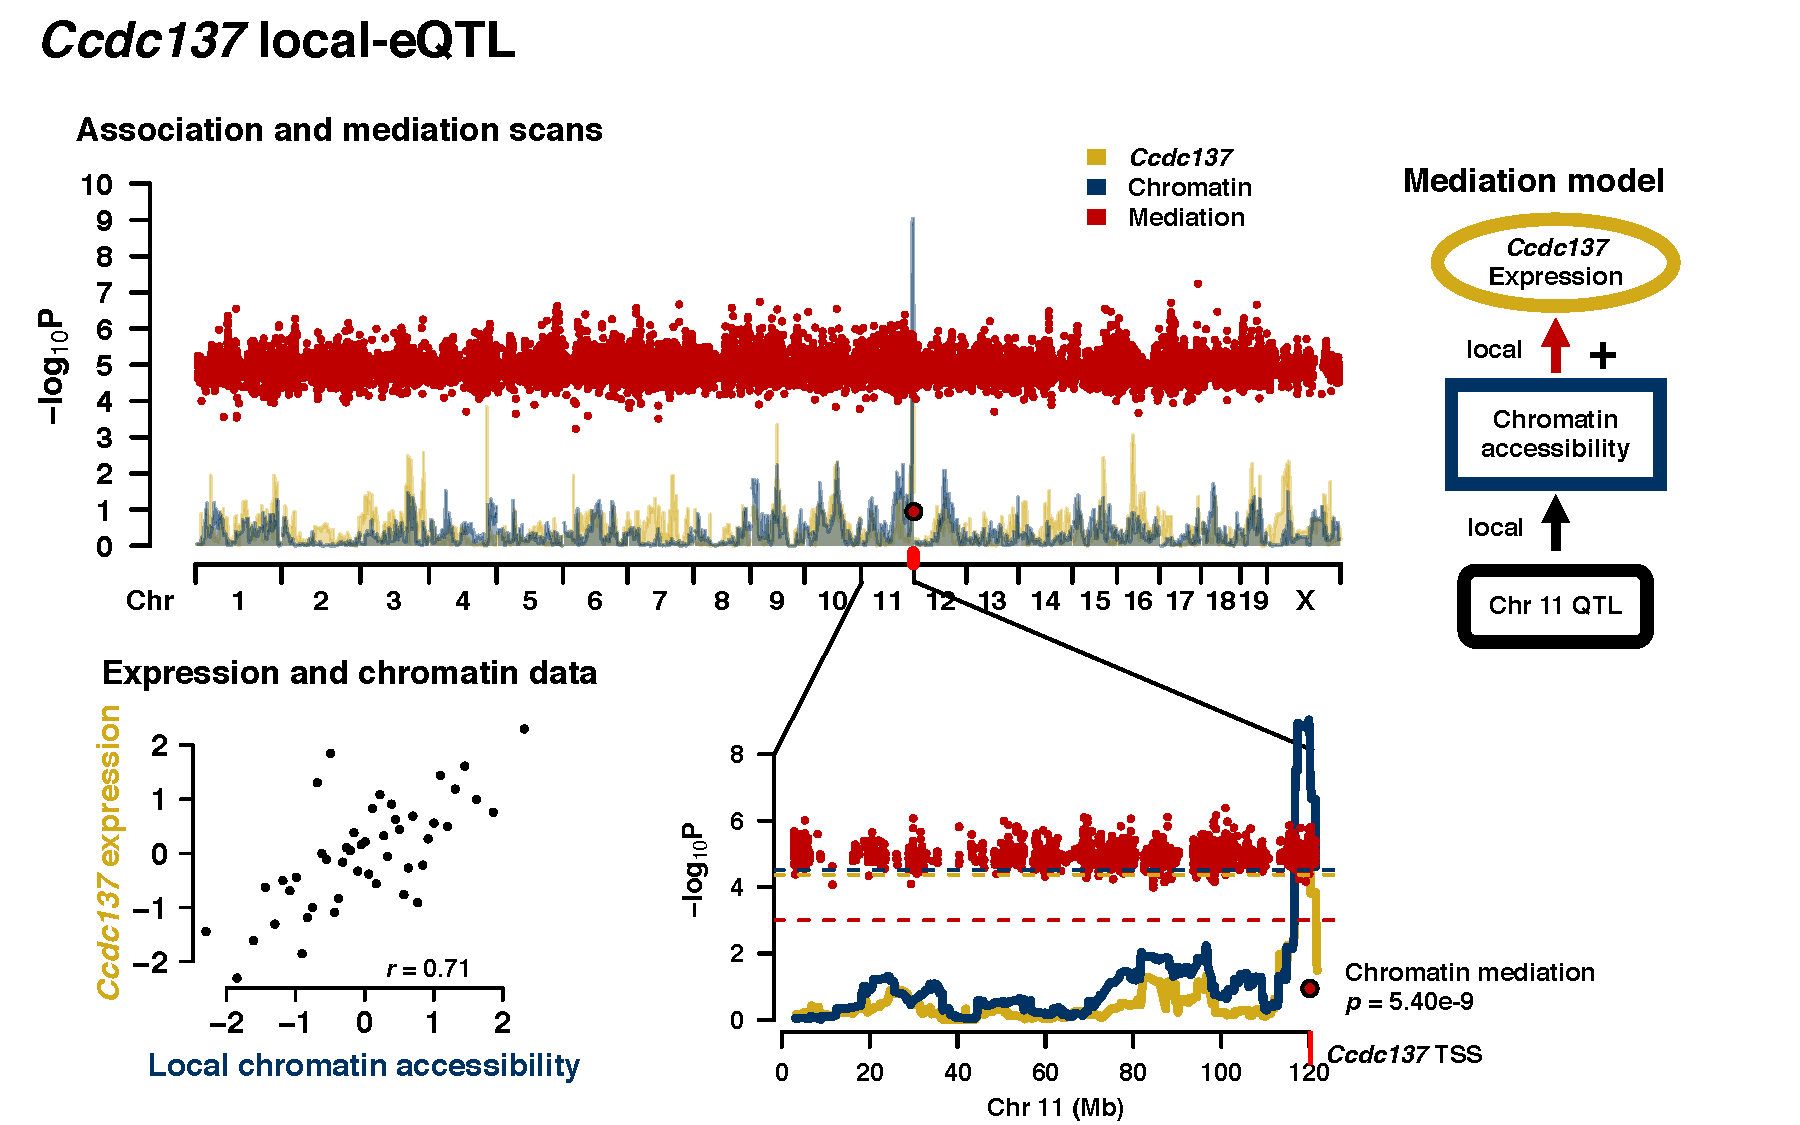
\includegraphics[width=\textwidth, trim={0in 0in 0in 0in}, clip]{figs/ccdc137_mediation.pdf}
\caption{\textbf{\textit{Ccdc137} local-eQTL is mediated by proximal chromatin accessibility.} \textit{Ccdc137} expression and the chromatin accessibility in the proximal region are highly correlated ($r = 0.71$). Genome scans for \textit{Ccdc137} expression (yellow), nearby chromatin accessibility (blue), and chromatin mediation of the \textit{Ccdc137} local-eQTL (red) in lung tissue. The local-eQTL and local-cQTL for the chromatin region at the TSS of \textit{Ccdc137} (red tick) are over-lapping. The steep drop in the statistical association, represented as logP, for the chromatin site in the mediation scan supports chromatin mediation of \textit{Ccdc137} expression, depicted as a simple graph in the topright. The QTL and mediation signals are detected at genome-wide significance. \label{fig:ccdc137_mediation}}
\end{figure*}

Founder allele effects that correlate across tissues can provide stronger confirmation of distal-QTL, even those with marginal significance. 
%Though fewer distal-QTL were significantly correlated across tissues in comparison to local-QTL (71 to 1,466 for eQTL and 2 to 213), potentially reflecting the reduced power to detect distal-QTL in this study, a number of genes were identified with unique patterns of distal-eQTL over the tissues, shown in \textbf{Figure \ref{fig:correlated_distal_eqtl}}.
For example, the Aldo-keto reductase family 1, member E1 (\textit{Akr1e1}; \textbf{Figure \ref{fig:correlated_distal_eqtl}A}) gene is located on chromosome 13 and had no local-eQTL detected in any of the tissues. Distal-eQTL for \textit{Akr1e1} were detected in all tissues that localize to the same distal region of chromosome 4. The founder allele effects of the distal-eQTL are all highly correlated, with A/J, B6, 129, and CAST being the more highly expressed alleles. The overall magnitude of expression varies significantly across the tissues, with liver and kidney having significantly higher expression than lung ($q = \num{1.63e-19}$ and $q = \num{4.40e-34}$, respectively).
%The distal-eQTL for \textit{Akr1e1} will be discussed further with the topic of mediation.
%As with local-QTL, correlated distal-eQTL can provide strong evidence that marginally significant QTL are valid. 
Another example is the Period circadian clock 2 (\textit{Per2}; \textbf{Figure \ref{fig:correlated_distal_eqtl}B}) gene, which possesses intra-chromosomal distal-eQTL that are detected in all three tissues that are approximately 100 Mb away from its TSS. Despite being detected with the highly lenient Method 2 (FDR $\leq$ 0.2), the founder allele effects are significantly correlated among the tissues, characterized by high expression with the NOD and PWK alleles present. Collectively, these findings provide strong validation for the distal-eQTL, which would commonly not be detected.

QTL analysis in multiple tissues also allows for the detection of tissue-specific distal-QTL. The Ring finger protein 13 (\textit{Rnf13}; \textbf{Figure \ref{fig:correlated_distal_eqtl}C}) gene was lowly expressed in all tissue but with a strong local-eQTL detected in liver. The multi-stage conditional regression approach, conditioning on the local-eQTL, detected a distal-eQTL on chromosome 12. Comparing the residuals after regressing out the local-eQTL and founder allele effects suggested that mice with B6 contributions at the distal locus had higher \textit{Rnf13} expression. In lung tissue, a distal-eQTL was detected on the X chromosome with a different founder allele pattern, notably high expression when A/J, B6, and PWK alleles were present, and low expression with NOD and NZO alleles. These examples demonstrate that analyzing multiple tissues can provide greater evidence of distal-QTL, as well as potentially identify tissue-specific genetic regulation.

\section{Mediation of eQTL}

Measurement of gene expression and chromatin accessibility data in the same mice and tissues enables the use of mediation analysis to elucidate the relationships between genotype, chromatin accessibility, and gene expressions. We assessed evidence for two mediation models of eQTL effects (\textbf{Figure \ref{fig:graph}}). First, we tested for proximal chromatin state as a mediator of the effect of local-eQTL on gene expression using an approach adapted from \cite{Chick2016} to detect mediation through chromatin accessibility of local-eQTL detected through Method 3 (genome-wide and chromosome-wide; see \textbf{Appendix C} for greater detail).  

%\subsection{Mediation of local-eQTL effects through proximal chromatin accessibility}

We found 30-68 local-eQTL showed evidence of mediation through proximal chromatin accessibility at genome-wide significance, and 70-181 at chromosome-wide significance (\textbf{Table \ref{tab:mediation}}). The coiled-coil domain containing 137 gene (\textit{Ccdc137}) is a strong example of mediation through local chromatin accessibility. \textbf{Figure \ref{fig:ccdc137_mediation}} includes the genome scans that identify local-QTL for \textit{Ccdc137} expression (eQTL) and a proximal chromatin accessibility window (cQTL). The red tick marks the TSS for \textit{Ccdc137}, which is highly proximal to both the eQTL and cQTL. The red dots represent the significance of the eQTL after conditioning on each chromatin region as a mediator. A large drop in eQTL significance at the location of the cQTL represents a strong mediation signal. A closer inspection of the region shows that the significance of the eQTL and cQTL are similar but notably stronger for chromatin, as expected by the proposed mediator model. 

Co-localization of eQTL and cQTL is not sufficient for mediation, shown in \textbf{Figure \ref{fig:colocalization}}. For both \textit{Hdhd3} in liver (\textbf{Figure \ref{fig:colocalization} [left]}) and the acyl-Coenzyme A binding domain containing 4 gene (\textit{Acbd4}) in kidney (\textbf{Figure \ref{fig:colocalization} [right]}), there are local-eQTL with a co-localizing cQTL. Comparing the statistical associations at the genomic locations of the eQTL and cQTL as well as the founder haplotype effects for both the eQTL and cQTL, the correspondence in both is better for \textit{Hdhd3} compared to \textit{Acbd4}. As with \textit{Ccdc137}, a strong mediation signal is detected for \textit{Hdhd3}, indicated by the decrease in the eQTL association when conditioning on the chromatin state. Mediation is not detected for \textit{Abcd4}, which is consistent with the genetic regulation of both gene and chromatin site not stemming from the same causal origin.

%\subsection{Mediation of distal-eQTL effects through proximal gene expression}

Next, we tested for evidence of expression levels of genes proximal to distal-eQTL acting as mediators, using an approach similar to \cite{Keller2018} for distal-eQTL detected through Method 1. 
%A related mediation model was used to identify genome-wide significant distal-eQTL that are mediated through the expression of proximal genes, as might be expected for a transcription factor with its own local-eQTL (\textbf{Figure \ref{fig:graph} B}). 
Eight genes were identified with mediated distal-eQTL (\textbf{Table \ref{tab:exmediation}}). As example, the distal-eQTL of cyclin Y-like 1 (\textit{Ccnyl1}) is mediated by the expression of zinc finger protein 979 (\textit{Zfp979}), a putative transcription factor (\textbf{Figure \ref{fig:ccnyl1_exmediation}}). The founder haplotype effects at the distal-eQTL of \textit{Ccnyl1} are highly correlated with the local-eQTL effects for \textit{Zfp979}, though with a reduction in overall strength, in accordance with the proposed mediation model.

\begin{figure*}[hp]
\renewcommand{\familydefault}{\sfdefault}\normalfont
\centering
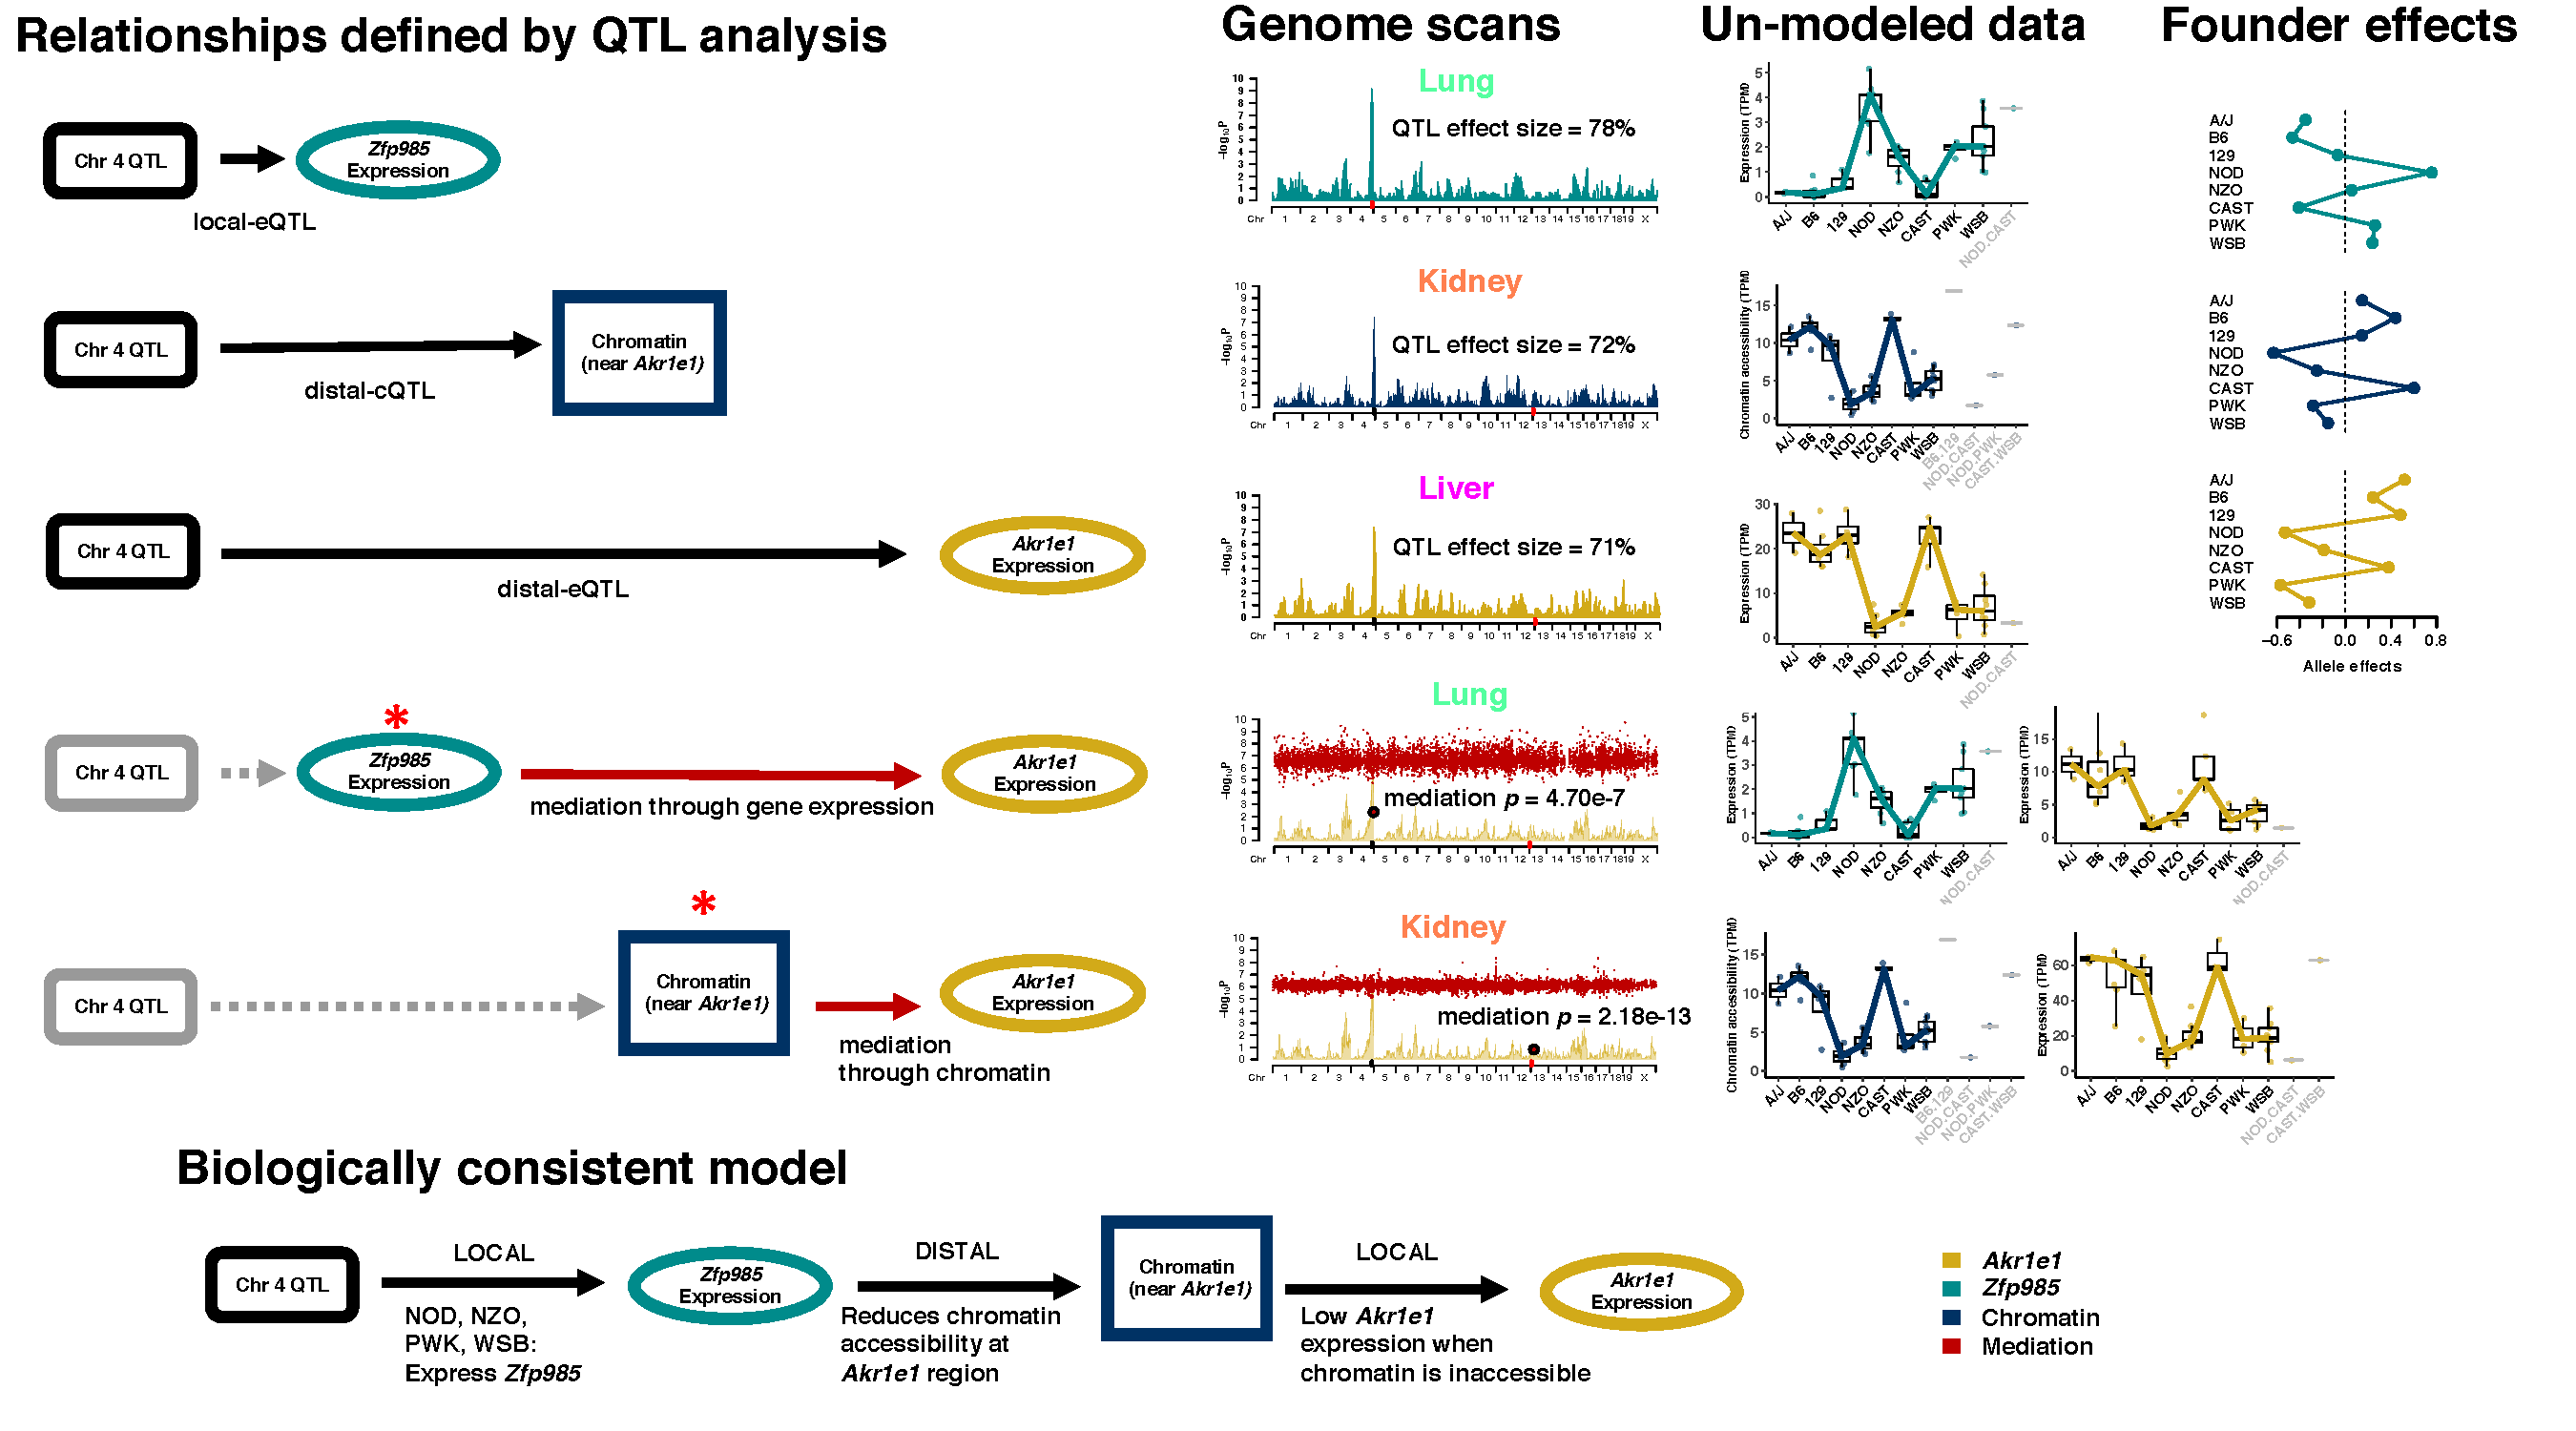
\includegraphics[width=\textwidth, trim={0in 0.1in 0in 0in}, clip]{figs/akr1e1_full_model.pdf}
\caption{\textbf{Complete mediation model for \textit{Akr1e1} distal-eQTL.}  The genetic regulation of \textit{Akr1e1} expression is reconstructed based on relationships observed across the three tissues. Distal-eQTL are detected in all tissues at similar levels of significance. A local-eQTL for \textit{Zfp985} that is proximal to the \textit{Akr1e1} distal-eQTL was observed in lung, and \textit{Zfp985} expression is detected as anti-correlated mediator of the distal-eQTL, consistent with \textit{Zfp985} suppressing \textit{Akr1e1} expression. The chromatin site proximal to the \textit{Akr1e1} TSS has a distal-cQTL detected in kidney. The chromatin accessibility at the site was found to be a significant correlated mediator of \textit{Akr1e1} expression. Combining associations across tissues supports a biological model whereby \textit{Zfp985}, expressed in mice with NOD, NZO, PWK, and WSB alleles, inhibits the proximal chromatin accessibility at the \textit{Akr1e1} TSS. QTL and mediation genome scans are included, along with sequence phenotypes as boxplots categorized according to most likely diplotype, and modeled founder effects fit as BLUPs. The relative magnitudes of the QTL effect sizes (estimated from Eq \ref{eq:effect_size}) and mediation significance are consistent with the proposed model, with \textit{Zfp985} local-eQTL > chromatin distal-eQTL > \textit{Akr1e1} distal-eQTL and chromatin mediation > mediation through \textit{Zfp985} expression.
\label{fig:akr1e1_full_model}}
\end{figure*}

\subsection{Proposed model for the genetic regulation of \textit{Akr1e1} expression}

As detailed above, \textit{Akr1e1} possesses a strong distal-eQTL, observed in all three tissues with significantly correlated founder effects. Additionally, we found that this effect is strongly mediated through Zinc finger protein 985 (\textit{Zfp985}) expression in lung. The \textit{Zfp985} TSS is located on chromosome 4 at 147.6 Mb, while the \textit{Akr1e1} distal-eQTL coordinates are 142.5 Mb, 143.2 Mb, and 148.6 Mb in liver, lung, and kidney, respectively (\textbf{Figure \ref{fig:akr1e1_exmediation}}). \textit{Akr1e1} and \textit{Zfp985} expression are negatively correlated ($r = -0.69$), which is consistent with \textit{Zfp985} inhibiting \textit{Akr1e1} expression. This same distal-eQTL and mediator relationship for \textit{Akr1e1} was observed in pancreatic islet tissue in DO mice \citep{Keller2018}.
The presence of distal genetic regulation for \textit{Akr1e1} was previously described in \cite{HamiltonWilliams2013}. The distal-eQTL we detect are highly proximal to their \textit{Idd9.2} region \citep{HamiltonWilliams2010}, originally defined as spanning 145.5-148.57 Mb of chromosome 4 and subsequently using NOD mice congenic with C57BL/10 (B10) introgressions \cite{HamiltonWilliams2013}. The B10 allele was found to be protective against the development of diabetes, characteristic of NOD mice. \textit{Akr1e1} is involved in glycogen metabolism and the larger \textit{Idd9} region harbors immune-related genes, implicating \textit{Akr1e1} and other genes located in and regulated by \textit{Idd9} as potential diabetes-related genes. 
Consistent with these studies, CC strains with NOD inheritance at the distal-eQTL have low expression of \textit{Akr1e1}. Genetic variation from B10 is not present in the CC, but the closely related B6 founder has high expression of \textit{Akr1e1} like B10. Similar to NOD, NZO, PWK, and WSB alleles result in low \textit{Akr1e1} expression, while A/J, 129, and CAST alleles join B6 as driving high expression (\textbf{Figure \ref{fig:akr1e1_full_model}}). Lowly expressed \textit{Zfp985} is a strong candidate for driving these effects on \textit{Akr1e1}.

Further elucidation of the genetic regulation of \textit{Akr1e1} was observed in kidney tissue, where a strong distal-cQTL is mapped to the \textit{Idd9.2} region for the chromatin site proximal to \textit{Akr1e1}. Based on the close proximities of the chromatin window to \textit{Akr1e1} and the distal-cQTL to the distal-eQTL, we mediated the distal-eQTL effect on the chromatin window, which was highly significant (permP = $\num{2.18e-13}$). The founder effects for the distal-cQTL are correlated with the distal-eQTL effects correlated ($r = 0.92$). The relative magnitudes of the QTL effect sizes and mediation p-values, shown in \textbf{Figure \ref{fig:akr1e1_relationships}}, support a causal model whereby \textit{Zfp985} expression reduces the expression of \textit{Akr1e1} by altering chromatin accessibility in the \textit{Akr1e1} proximal promoter region (\textbf{Figure \ref{fig:akr1e1_full_model}}). 

\subsection{Overview of QTL and mediation analyses}

All QTL and mediation results for all three tissues are depicted in \textbf{Figure \ref{fig:circos_plot}}. Notably, local-QTL and chromatin mediation are not evenly distributed across the genome, but tend to aggregate in pockets. In particular, there is a high concentration of cQTL and chromatin mediation detected along chromosome 17, observed across all three tissues, which happens to correspond to the immune-related major histocompatibility (MHC) region in mouse. However, we note that most of the chromatin-mediated genes in this region are not histocompatibility genes (\textbf{Tables SXX}). The patterns of distal-QTL and gene mediation appear to be tissue-specific, though there are consistent regions observed across the tissues, such as the \textit{Idd9} region \citep{HamiltonWilliams2010} of chromosome 4, which contains multiple zinc finger proteins and regulates genes such as \textit{Akr1e1} and \textit{Ccnyl1}. Previously discussed genes are highlighted for each tissue.

\begin{figure*}[h!]
\renewcommand{\familydefault}{\sfdefault}\normalfont
\centering
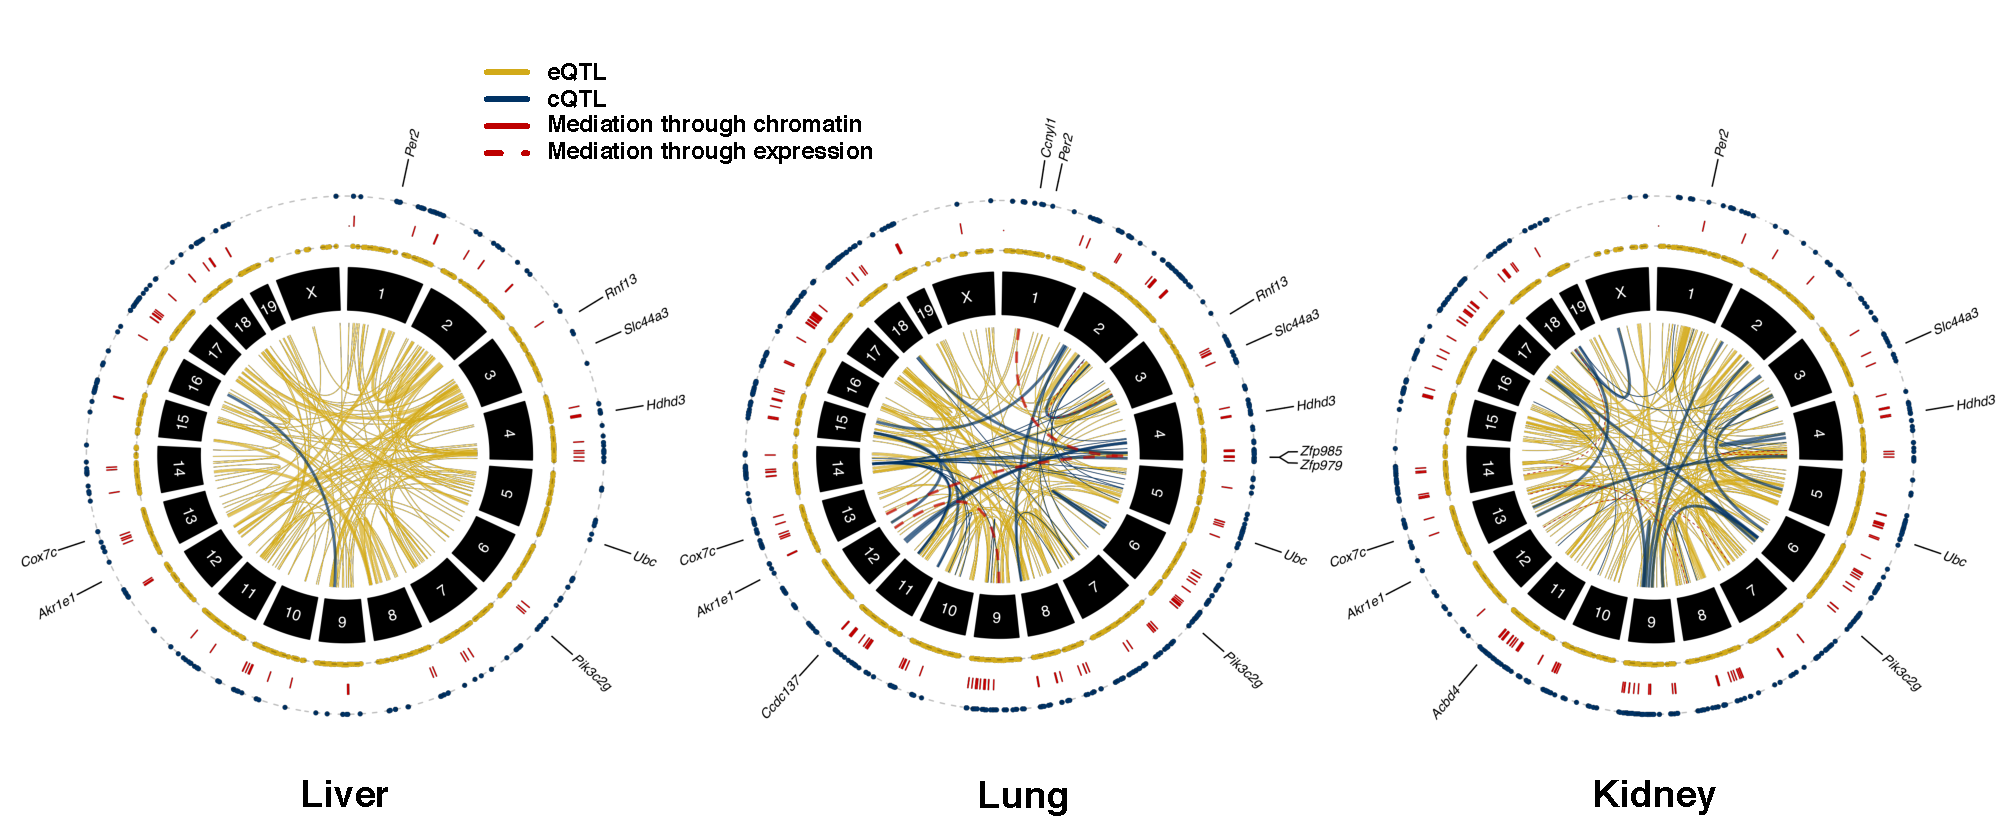
\includegraphics[width=\textwidth, trim={0in 0in 0in 0in}, clip]{figs/circos_over_tissues.pdf}
\caption{\textbf{Summaries of eQTL, cQTL, and mediation analyses.} Circos plots of eQTL (yellow), cQTL (blue), and mediation (red) in lung, liver, and kidney. The two outer rings of dots represent local-eQTL and local-cQTL detected by Method 3 at chromosome-wide significance, with red lines between connecting genes and chromatin sites for which chromatin mediation was detected. The inner circle contains connections representing distal-eQTL, distal-cQTL, and gene-gene mediation from Method 1. Thick lines represent QTL and mediators with permutation-based p-value (permP) $< \num{1e-5}$. The detected signals are primarily local, which also tend to be stronger than the observed distal signals. Fewer QTL and mediators are detected in liver tissue. 
%Chromosome 17 has the most concentrated chromatin mediation signal across the three tissues. 
Genes highlighted previously, such as \textit{Akr1e1}, are indicated at their genomic coordinates.
\label{fig:circos_plot}}
\end{figure*}

